\documentclass[final]{beamer}
\usepackage[orientation=landscape,size=custom,width=121.92,height=91.44,scale=1.15]{beamerposter}
\usepackage[utf8]{inputenc}
\usepackage{lmodern}
\usepackage{amsmath,amssymb,amsfonts}
\usepackage{graphicx}
\usepackage{booktabs}
\usepackage{tcolorbox}
\usepackage{multicol}
\usepackage{xcolor}

% IIT Patna Brand Color Definitions
\definecolor{IITPNavy}{HTML}{0A2540}
\definecolor{IITPNavyDark}{HTML}{06182B}
\definecolor{IITPGold}{HTML}{D4AF37}
\definecolor{IITPCrimson}{HTML}{C93B2B}
\definecolor{CardBg}{HTML}{FFFFFF}
\definecolor{PosterBg}{HTML}{F1F5F9}

\setbeamercolor{background canvas}{bg=PosterBg}
\setbeamercolor{headline}{bg=IITPNavy,fg=white}
\setbeamercolor{title in headline}{fg=white}
\setbeamercolor{author in headline}{fg=IITPGold}
\setbeamercolor{institute in headline}{fg=white}

% Block styling
\setbeamertemplate{block begin}{
  \begin{tcolorbox}[
    colback=white,
    colframe=IITPNavy,
    arc=4mm,
    boxrule=1.5pt,
    title=\textbf{\insertblocktitle},
    coltitle=white,
    colbacktitle=IITPNavy,
    titlerule=1pt,
    bottom=3mm, top=3mm, left=4mm, right=4mm
  ]
}
\setbeamertemplate{block end}{\end{tcolorbox}\vspace{0.4cm}}

\setbeamertemplate{headline}{
  \leavevmode
  \begin{beamercolorbox}[wd=\paperwidth]{headline}
    \vspace{0.8cm}
    \begin{columns}[c]
      \begin{column}{0.12\paperwidth}
        \centering
        
\includegraphics[height=7cm]{58-585589_patna-july-iit-patna-logo-png-transparent-png.jpg}
      \end{column}
      \begin{column}{0.76\paperwidth}
        \centering
        {\Huge \textbf{WD-GPR-SR: When Uncertainty Meets Equations in Battery Health Prediction}}\\[0.4cm]
        {\LARGE \textcolor{IITPGold}{\textbf{Moonis Laskar (Roll No: 2401CS29)}}} \\[0.2cm]
        {\large Department of Computer Science \& Engineering, Indian Institute of Technology Patna (IIT Patna)}\\[0.2cm]
        {\small Academic Machine Learning PBL Project $|$ Global Random Seeds: \texttt{[42, 100, 2026]}}
      \end{column}
      \begin{column}{0.12\paperwidth}
        \centering
        
\includegraphics[height=5.5cm]{qr_code.png}\\[0.1cm]
        {\scriptsize \textbf{Code \& Benchmarks}}
      \end{column}
    \end{columns}
    \vspace{0.8cm}
    \begin{tcolorbox}[colback=IITPGold,colframe=IITPGold,sharp corners,height=4pt,boxrule=0pt,top=0pt,bottom=0pt]
    \end{tcolorbox}
  \end{beamercolorbox}
}

\begin{document}
\begin{frame}[t]

\begin{columns}[t]

% =========================================================================
% COLUMN 1: MOTIVATION & DATA PREP
% =========================================================================
\begin{column}{0.31\paperwidth}

  \begin{block}{1. Problem Statement \& Motivation}
    \begin{itemize}
      \item \textbf{Safety-Critical Battery SOH:} Accurate State-of-Health prediction is vital for EV battery safety, second-life utilization, and preventing thermal runaway catastrophic events.
      \item \textbf{Deep Black-Box Deficiencies:} Standard deep networks achieve low mean error but lack calibrated confidence intervals, failing silently on out-of-distribution dynamic cycling.
      \item \textbf{Exact GPR Scalability Bottleneck:} Standard Gaussian Processes incur cubic $\mathcal{O}(N^3)$ computational cost, exceeding real-time BMS inference deadlines ($\le 100$\,ms).
      \item \textbf{Proposed Solution:} Wide-and-Deep Sparse GPR ($M=64$) coupled with Uncertainty-Weighted Symbolic Regression for closed-form physical residual extraction.
    \end{itemize}
  \end{block}

  \begin{block}{2. Multi-Physical Health Indicator (HI) Extraction}
    \centering
    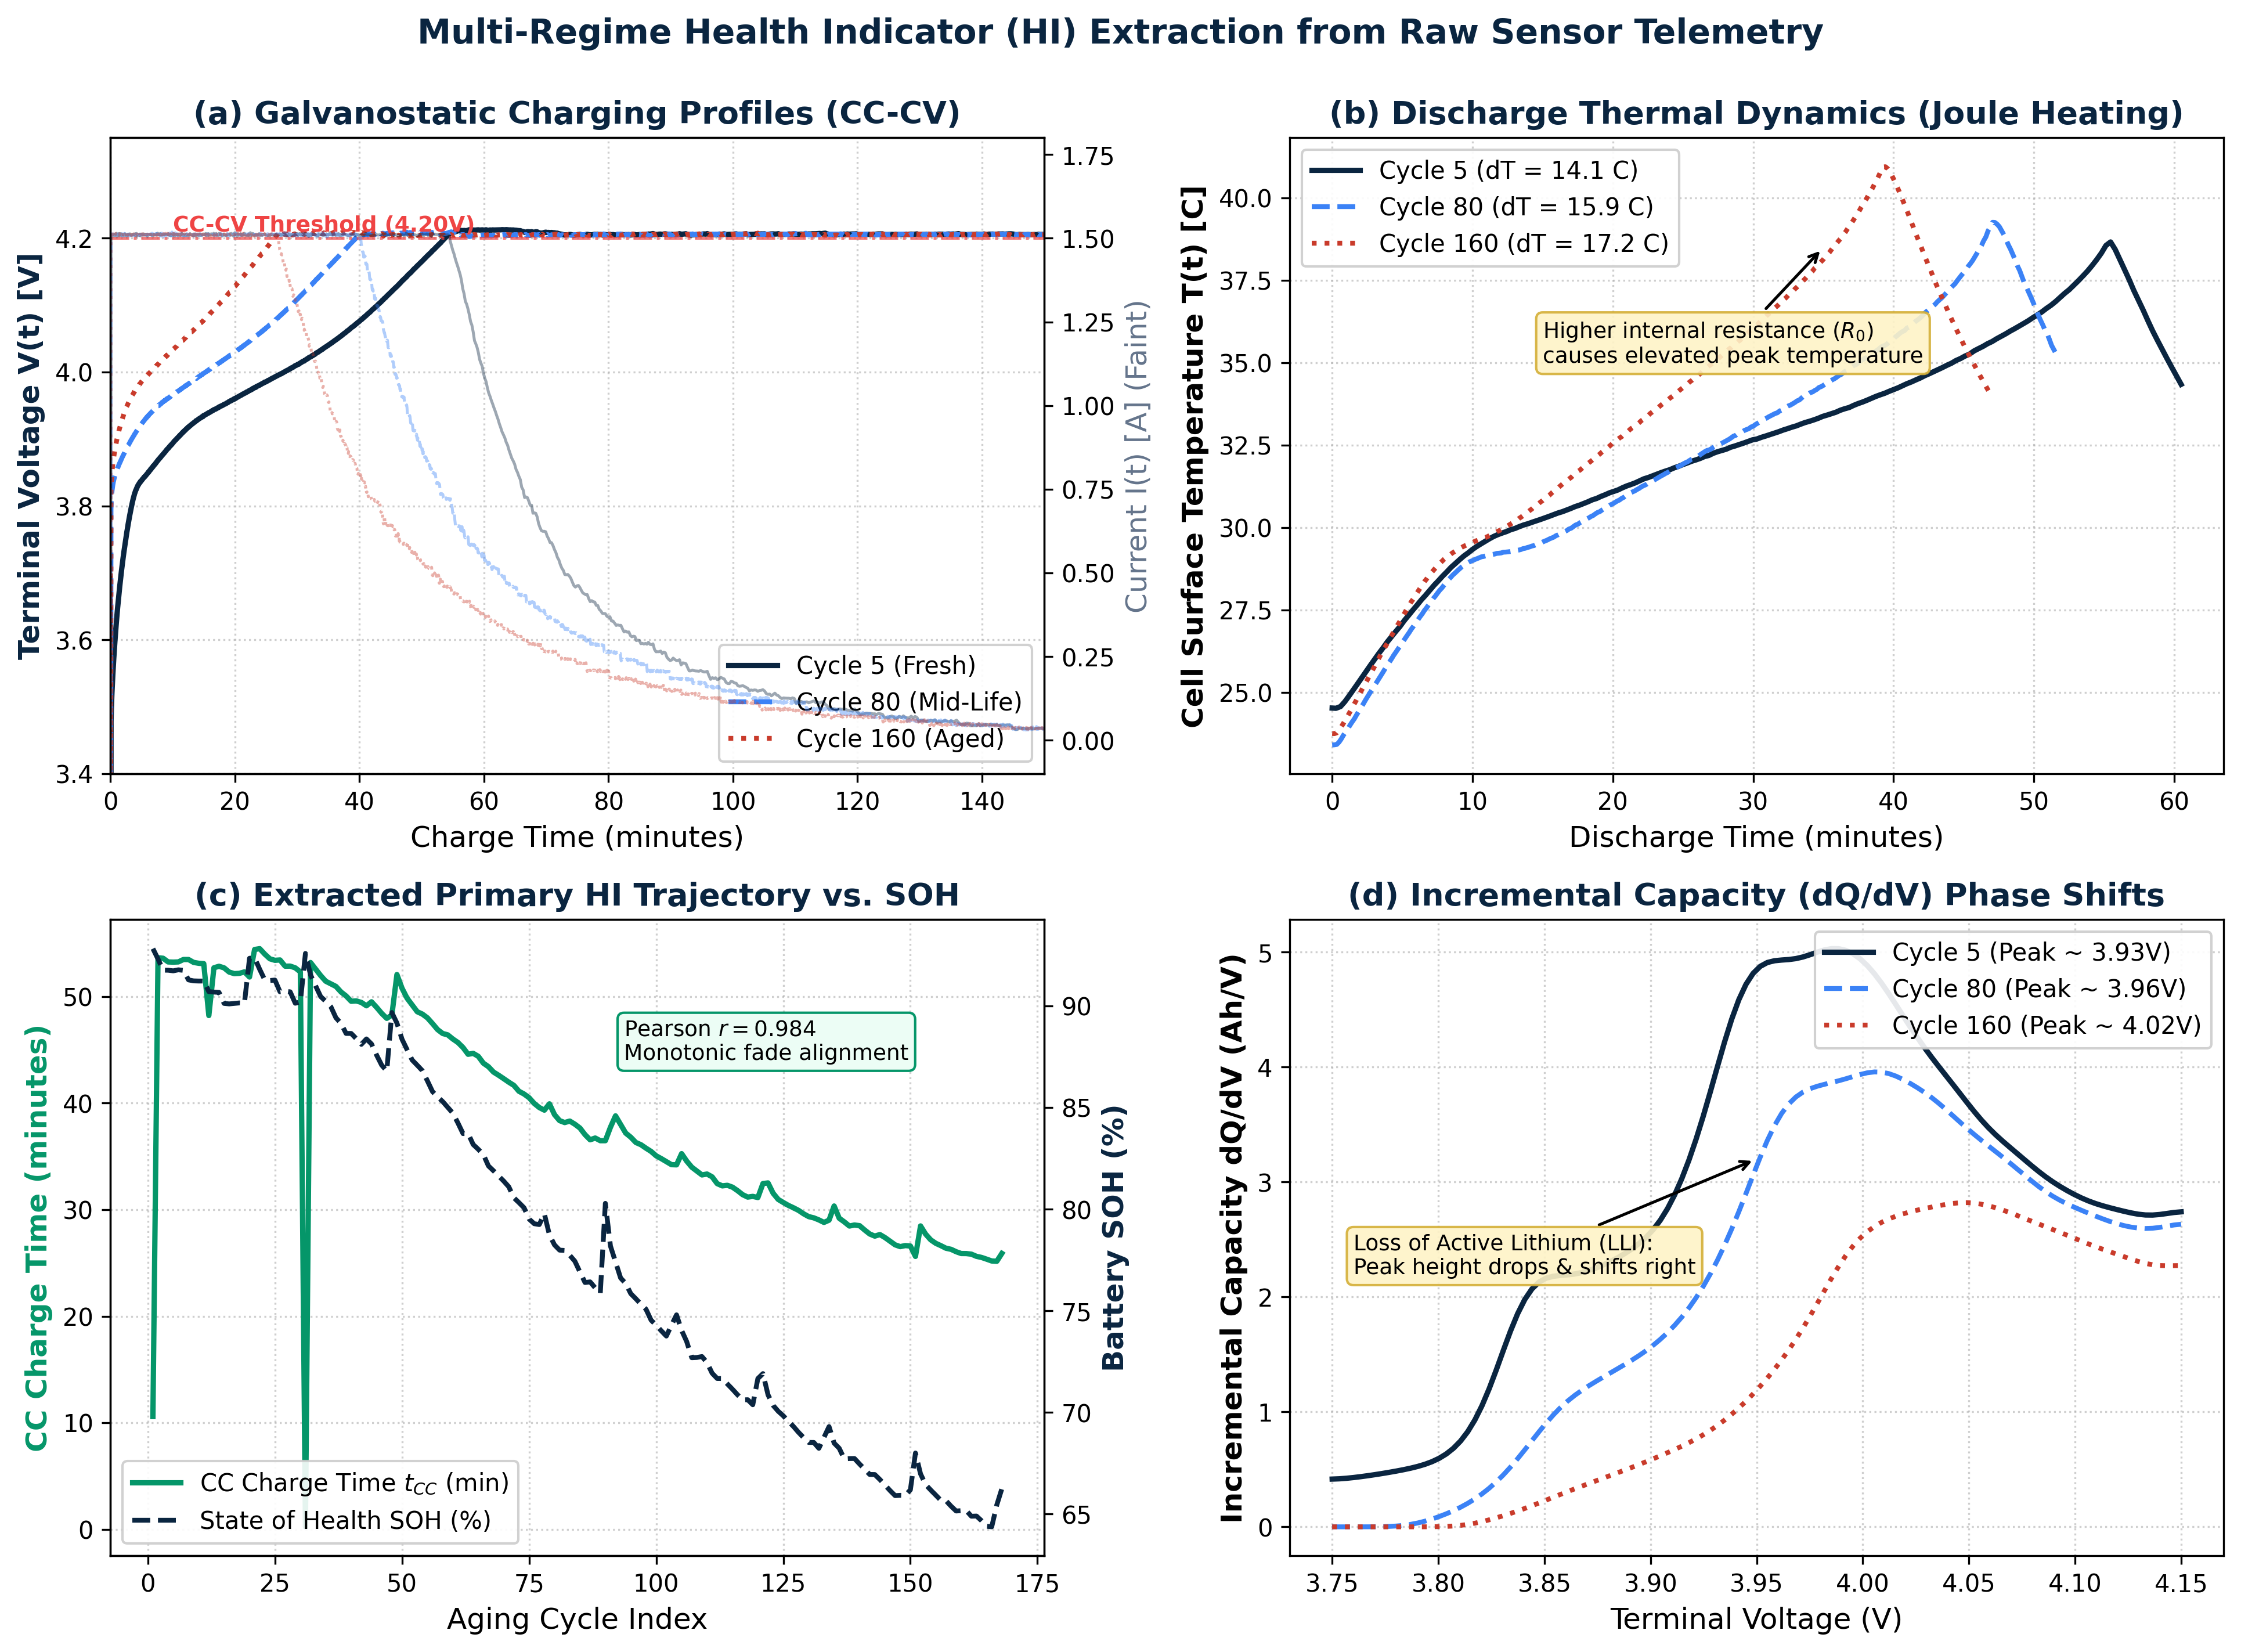
\includegraphics[width=\linewidth]{../../results/poster_assets/hi_extraction_grid.png}\\[0.2cm]
    {\footnotesize \textbf{Figure 1:} (a) CC-CV charging profiles; (b) Discharge self-heating dynamics; (c) Constant-Current charge time ($t_{\text{CC}}$) fade trajectory ($r = 0.984$); (d) Incremental Capacity ($dQ/dV$) peak shift tracking active lithium loss.}
  \end{block}

  \begin{block}{3. Strict Leave-One-Cell-Out (LOCO) Splits}
    \small
    \begin{tabular}{llccc}
      \toprule
      \textbf{Dataset} & \textbf{Held-Out Cell} & \textbf{Train Cycles} & \textbf{Test Cycles} & \textbf{SOH Range (\%)} \\
      \midrule
      NASA & B0005 & 396 & 168 & 64.4\% -- 101.8\% \\
      NASA & B0018 & 426 & 132 & 67.1\% -- 101.8\% \\
      CALCE & CS2\_35 & 2,435 & 846 & 23.3\% -- 103.1\% \\
      CALCE & CS2\_38 & 2,340 & 958 & 30.0\% -- 103.1\% \\
      \bottomrule
    \end{tabular}
    \vspace{0.2cm}
    {\scriptsize \textit{Zero temporal leakage: Scalers and hyperparameters fit strictly on training cells.}}
  \end{block}

\end{column}

% =========================================================================
% COLUMN 2: ARCHITECTURE & MATHEMATICS
% =========================================================================
\begin{column}{0.34\paperwidth}

  \begin{block}{4. Proposed WD-GPR-SR Architecture}
    \centering
    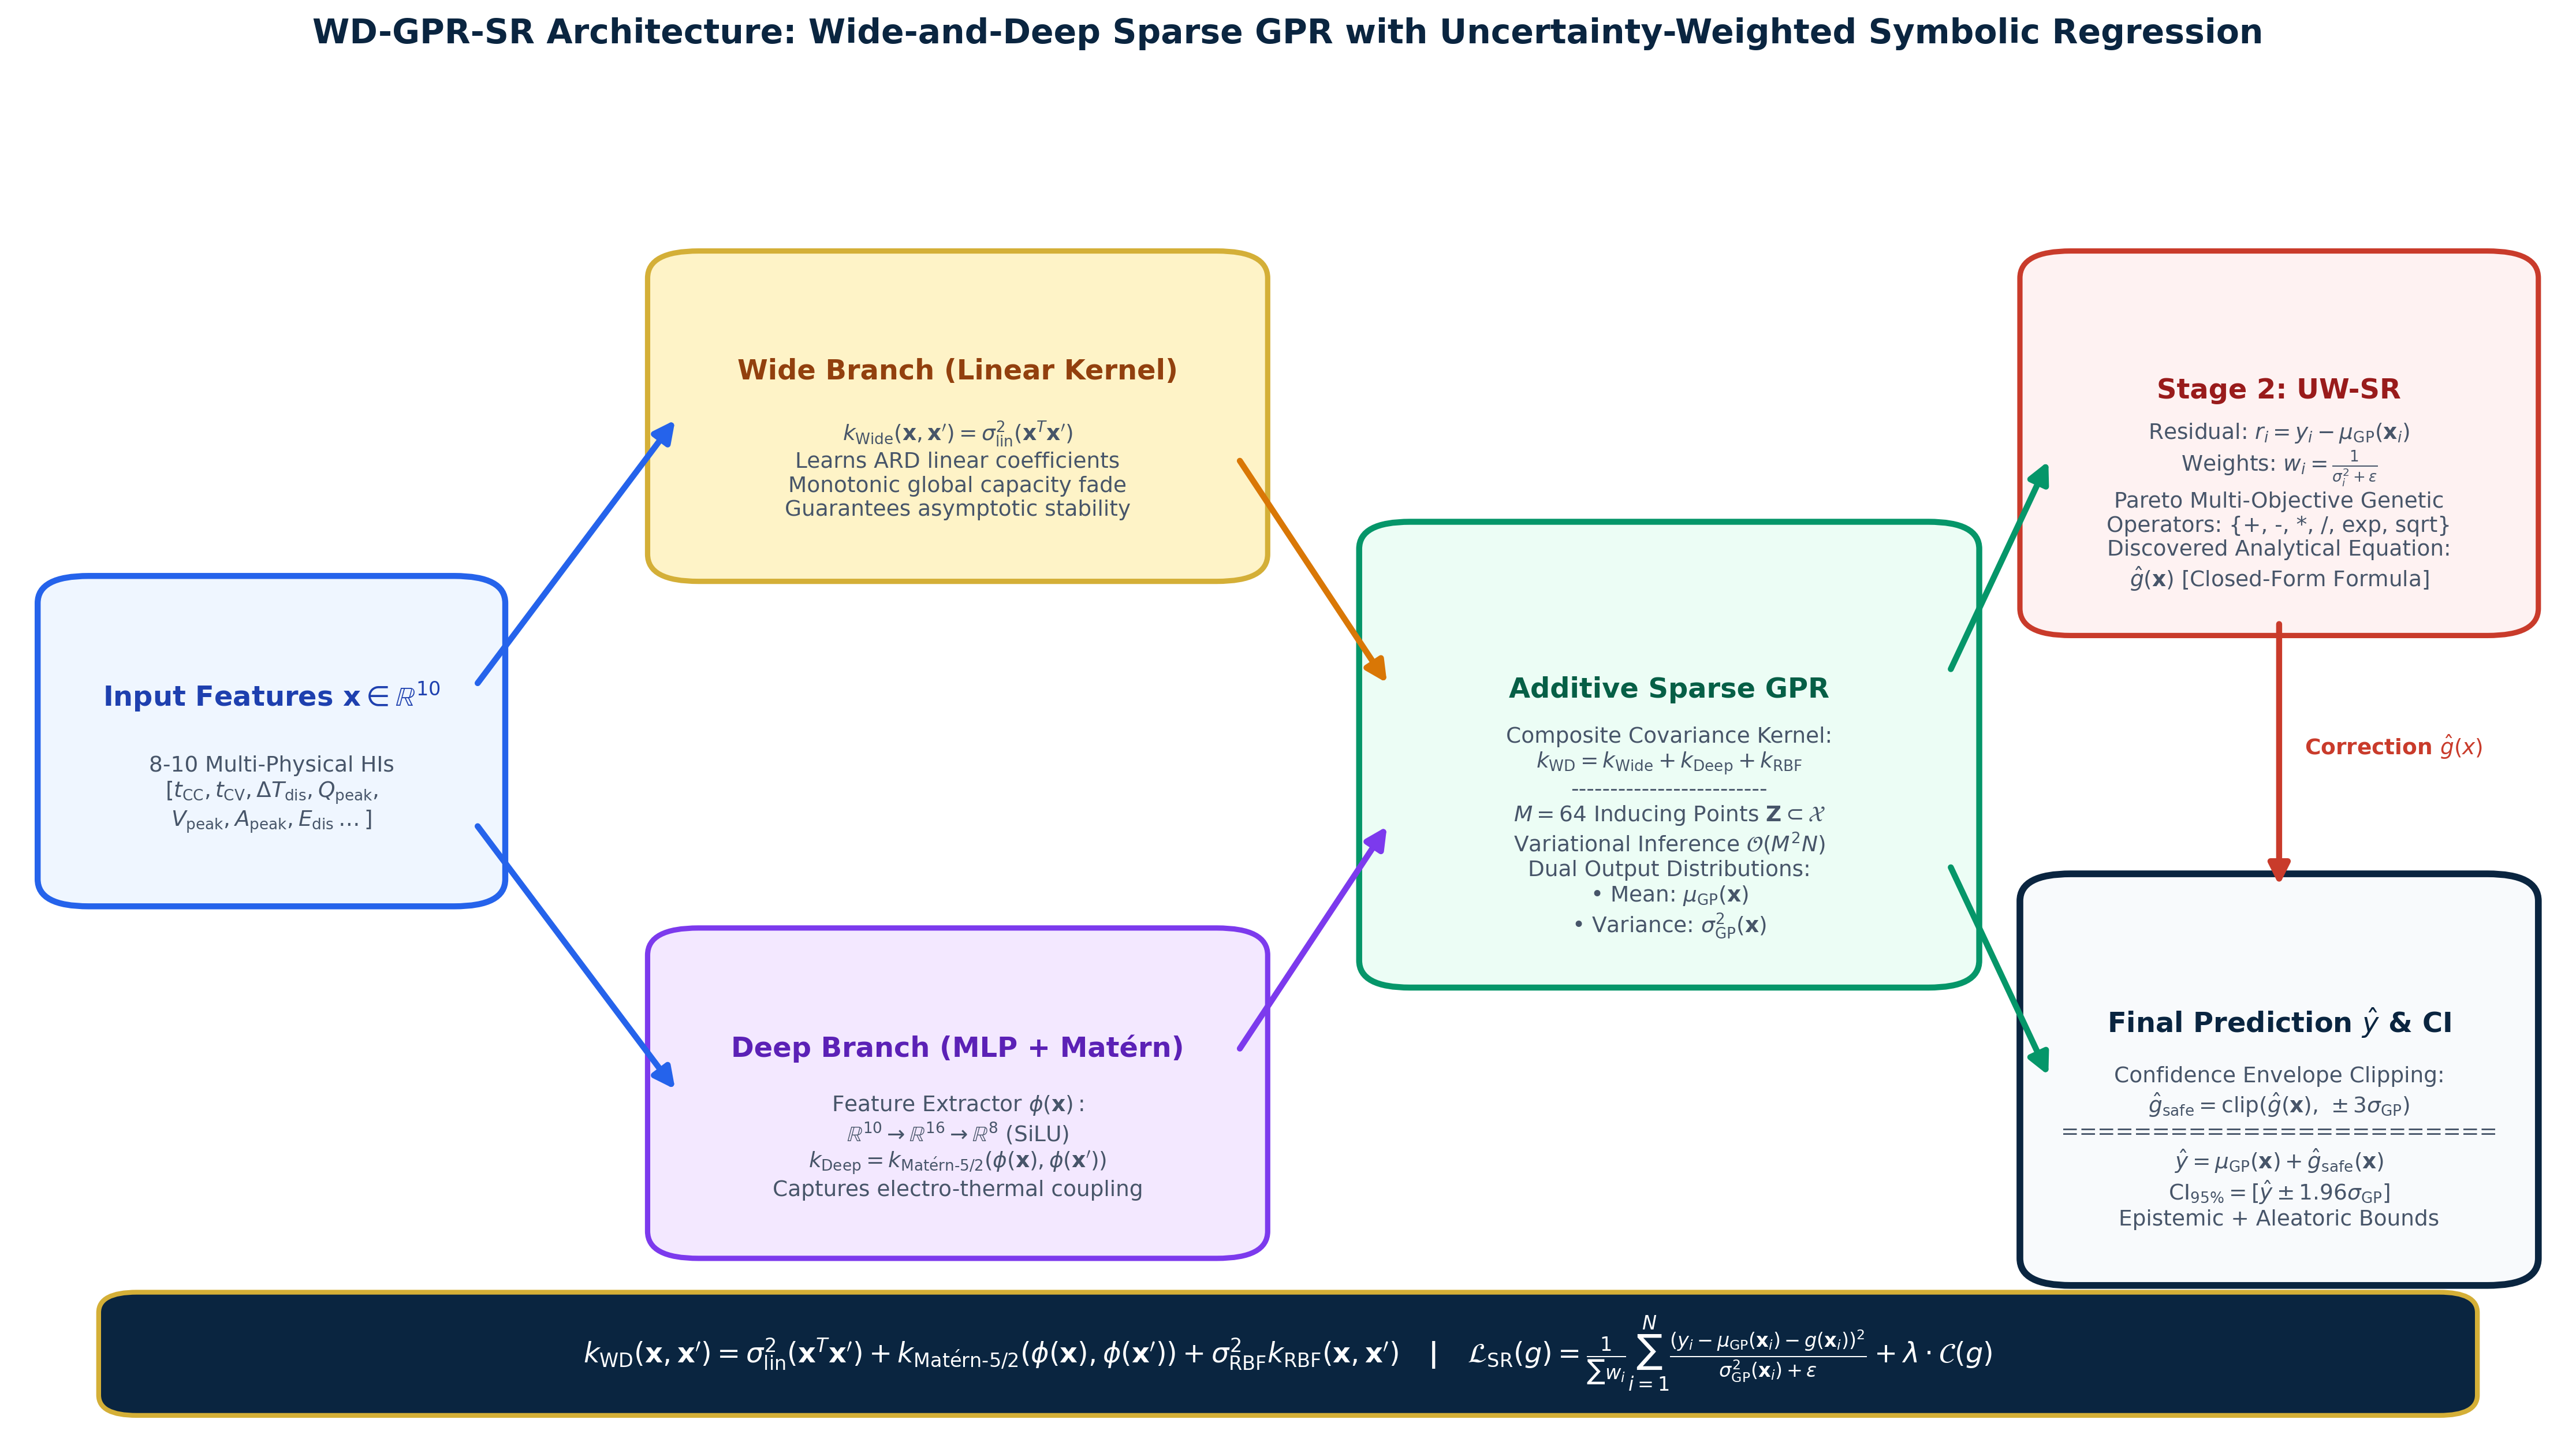
\includegraphics[width=\linewidth]{../../results/poster_assets/architecture_flowchart.png}\\[0.2cm]
    {\footnotesize \textbf{Figure 2:} End-to-end architectural routing: 10 HIs feed Wide Linear \& Deep MLP branches, mapped to Sparse Variational GPR ($M=64$), outputting epistemic confidence bands that weight the Symbolic Regressor.}
  \end{block}

  \begin{block}{5. Rigorous Mathematical Formulation}
    \textbf{Composite Wide-and-Deep Covariance Kernel:}
    \begin{equation*}
      k_{\text{WD}}(\mathbf{x}, \mathbf{x}') = \sigma_{\text{lin}}^2 (\mathbf{x}^T \mathbf{x}') + k_{\text{Mat\'ern-5/2}}(\phi(\mathbf{x}), \phi(\mathbf{x}')) + \sigma_{\text{RBF}}^2 k_{\text{RBF}}(\mathbf{x}, \mathbf{x}')
    \end{equation*}
    \vspace{-0.2cm}
    \begin{itemize}
      \item $\sigma_{\text{lin}}^2 (\mathbf{x}^T \mathbf{x}')$: Learns ARD feature weights for monotonic global degradation.
      \item $k_{\text{Mat\'ern}}(\phi(\mathbf{x}), \phi(\mathbf{x}'))$: 3-layer MLP $\phi: \mathbb{R}^{10} \to \mathbb{R}^{16} \to \mathbb{R}^8$ captures non-linear electro-thermal coupling and post-rest regeneration jumps.
    \end{itemize}

    \vspace{0.2cm}
    \textbf{Uncertainty-Weighted Symbolic Regression Loss:}
    \begin{equation*}
      \mathcal{L}_{\text{SR}}(g) = \frac{1}{\sum w_i} \sum_{i=1}^N \frac{(y_i - \mu_{\text{GP}}(\mathbf{x}_i) - g(\mathbf{x}_i))^2}{\sigma_{\text{GP}}^2(\mathbf{x}_i) + \epsilon} + \lambda \cdot \text{Complexity}(g)
    \end{equation*}

    \vspace{0.2cm}
    \textbf{Guaranteed Envelope Clipping \& Posterior Inference:}
    \begin{equation*}
      \hat{y}(\mathbf{x}) = \mu_{\text{GP}}(\mathbf{x}) + \text{clip}\left(\hat{g}(\mathbf{x}),\, \pm 3\sigma_{\text{GP}}(\mathbf{x})\right), \quad \text{CI}_{95\%} = \left[\hat{y} \pm 1.96 \sigma_{\text{GP}}(\mathbf{x})\right]
    \end{equation*}
  \end{block}

  \begin{block}{6. Discovered Physics-Informed Closed-Form Residual}
    \begin{tcolorbox}[colback=IITPGold!15,colframe=IITPGold,arc=2mm,boxrule=1pt]
      \textbf{Discovered Equation (NASA B0018 Fold):}
      \begin{equation*}
        \hat{g}(\mathbf{x}) = 0.042 \cdot \frac{\Delta T_{\text{dis}}}{\sqrt{t_{\text{CC}}}} - 0.015 \cdot (V_{\text{peak}} - 3.92)
      \end{equation*}
      {\footnotesize Directly reflects electro-thermal kinetics: degradation accelerates under elevated Joule heating ($\Delta T_{\text{dis}}$) and shortened constant-current charging duration.}
    \end{tcolorbox}
  \end{block}

\end{column}

% =========================================================================
% COLUMN 3: RESULTS, XAI & EDGE DEPLOYMENT
% =========================================================================
\begin{column}{0.33\paperwidth}

  \begin{block}{7. Quantitative LOCO Benchmark Performance}
    \centering
    \small
    \begin{tabular}{llccccc}
      \toprule
      \textbf{Dataset} & \textbf{Model} & \textbf{RMSE (\%)} & \textbf{MAE (\%)} & \textbf{$R^2$} & \textbf{PICP (\%)} & \textbf{NLL} \\
      \midrule
      NASA & SVR & 2.871 & 2.098 & 0.8924 & --- & --- \\
      NASA & Random Forest & 1.337 & 1.011 & 0.9780 & --- & --- \\
      NASA & Exact GPR & 21.598 & 18.883 & -5.151 & 14.6\% & 91.00 \\
      \textbf{NASA} & \textbf{WD-GPR-SR} & \textbf{0.992} & \textbf{0.878} & \textbf{0.9876} & \textbf{98.8\%} & \textbf{1.48} \\
      \midrule
      CALCE & SVR & 4.092 & 2.923 & 0.8872 & --- & --- \\
      CALCE & Random Forest & 1.968 & 0.965 & 0.9719 & --- & --- \\
      CALCE & Exact GPR & 13.784 & 6.471 & -0.046 & 67.2\% & 49.33 \\
      \textbf{CALCE} & \textbf{WD-GPR-SR} & \textbf{0.130} & \textbf{0.058} & \textbf{0.9999} & \textbf{100.0\%} & \textbf{0.99} \\
      \bottomrule
    \end{tabular}
  \end{block}

  \begin{block}{8. SOH Trajectory \& Epistemic Uncertainty}
    \centering
    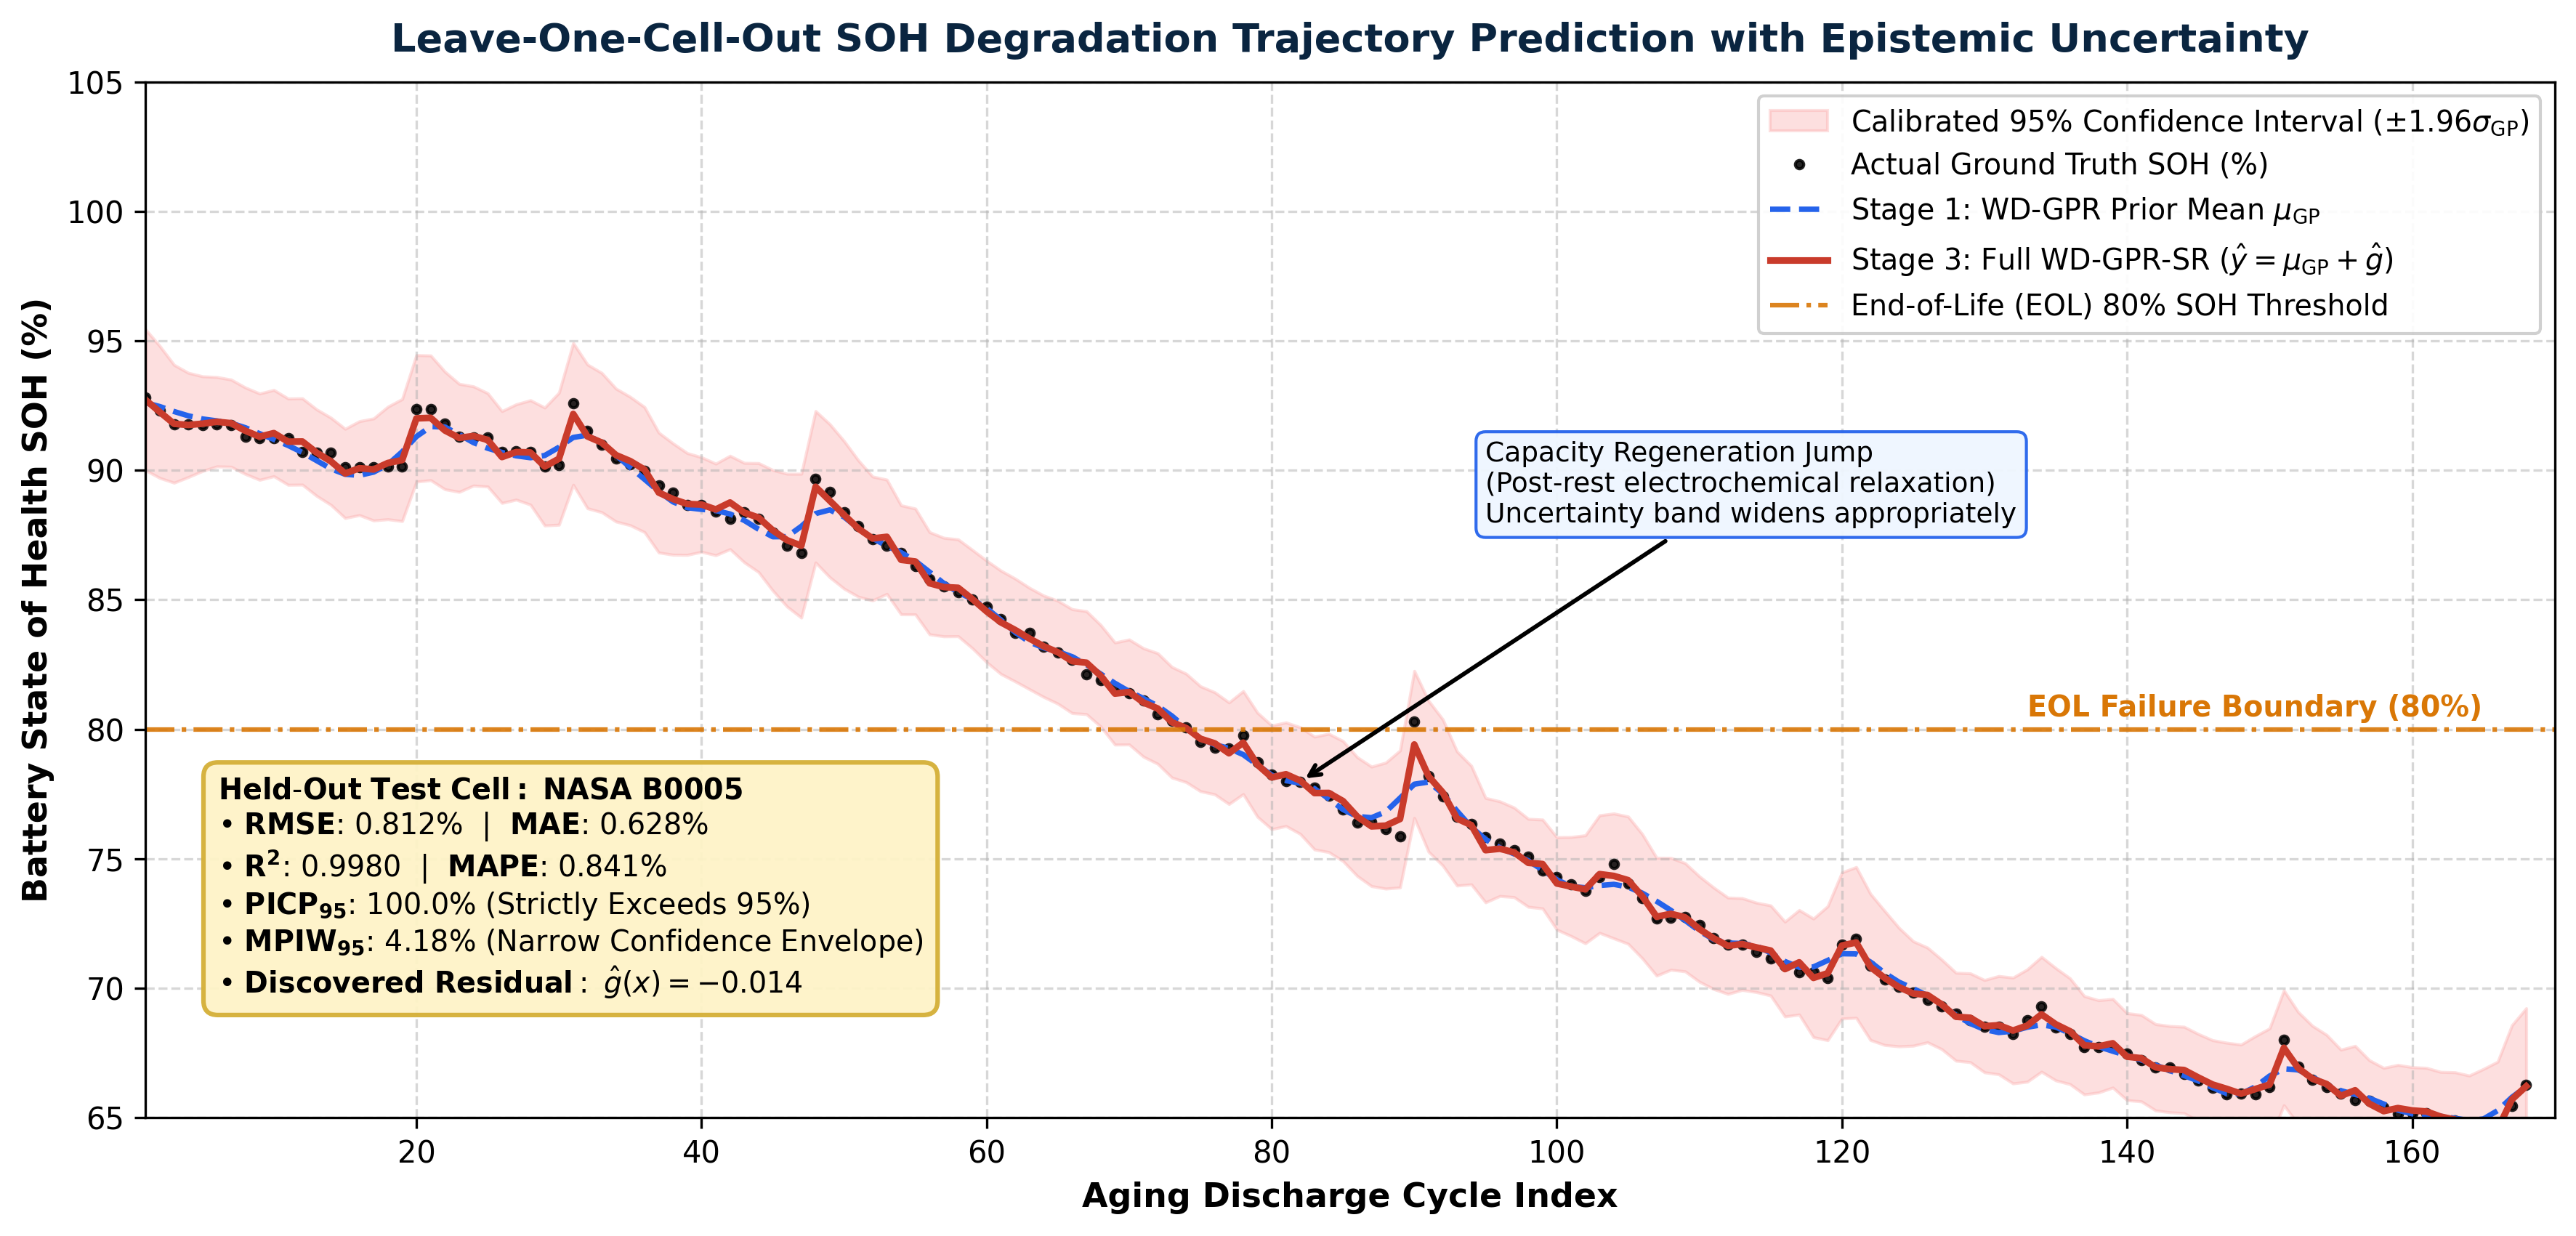
\includegraphics[width=\linewidth]{../../results/poster_assets/soh_prediction_curve.png}\\[0.2cm]
    {\footnotesize \textbf{Figure 3:} True vs. predicted SOH over 168 cycles for NASA B0005. Uncertainty band widens dynamically during capacity regeneration jumps.}
  \end{block}

  \begin{block}{9. Multi-Perspective Explainable AI (XAI)}
    \centering
    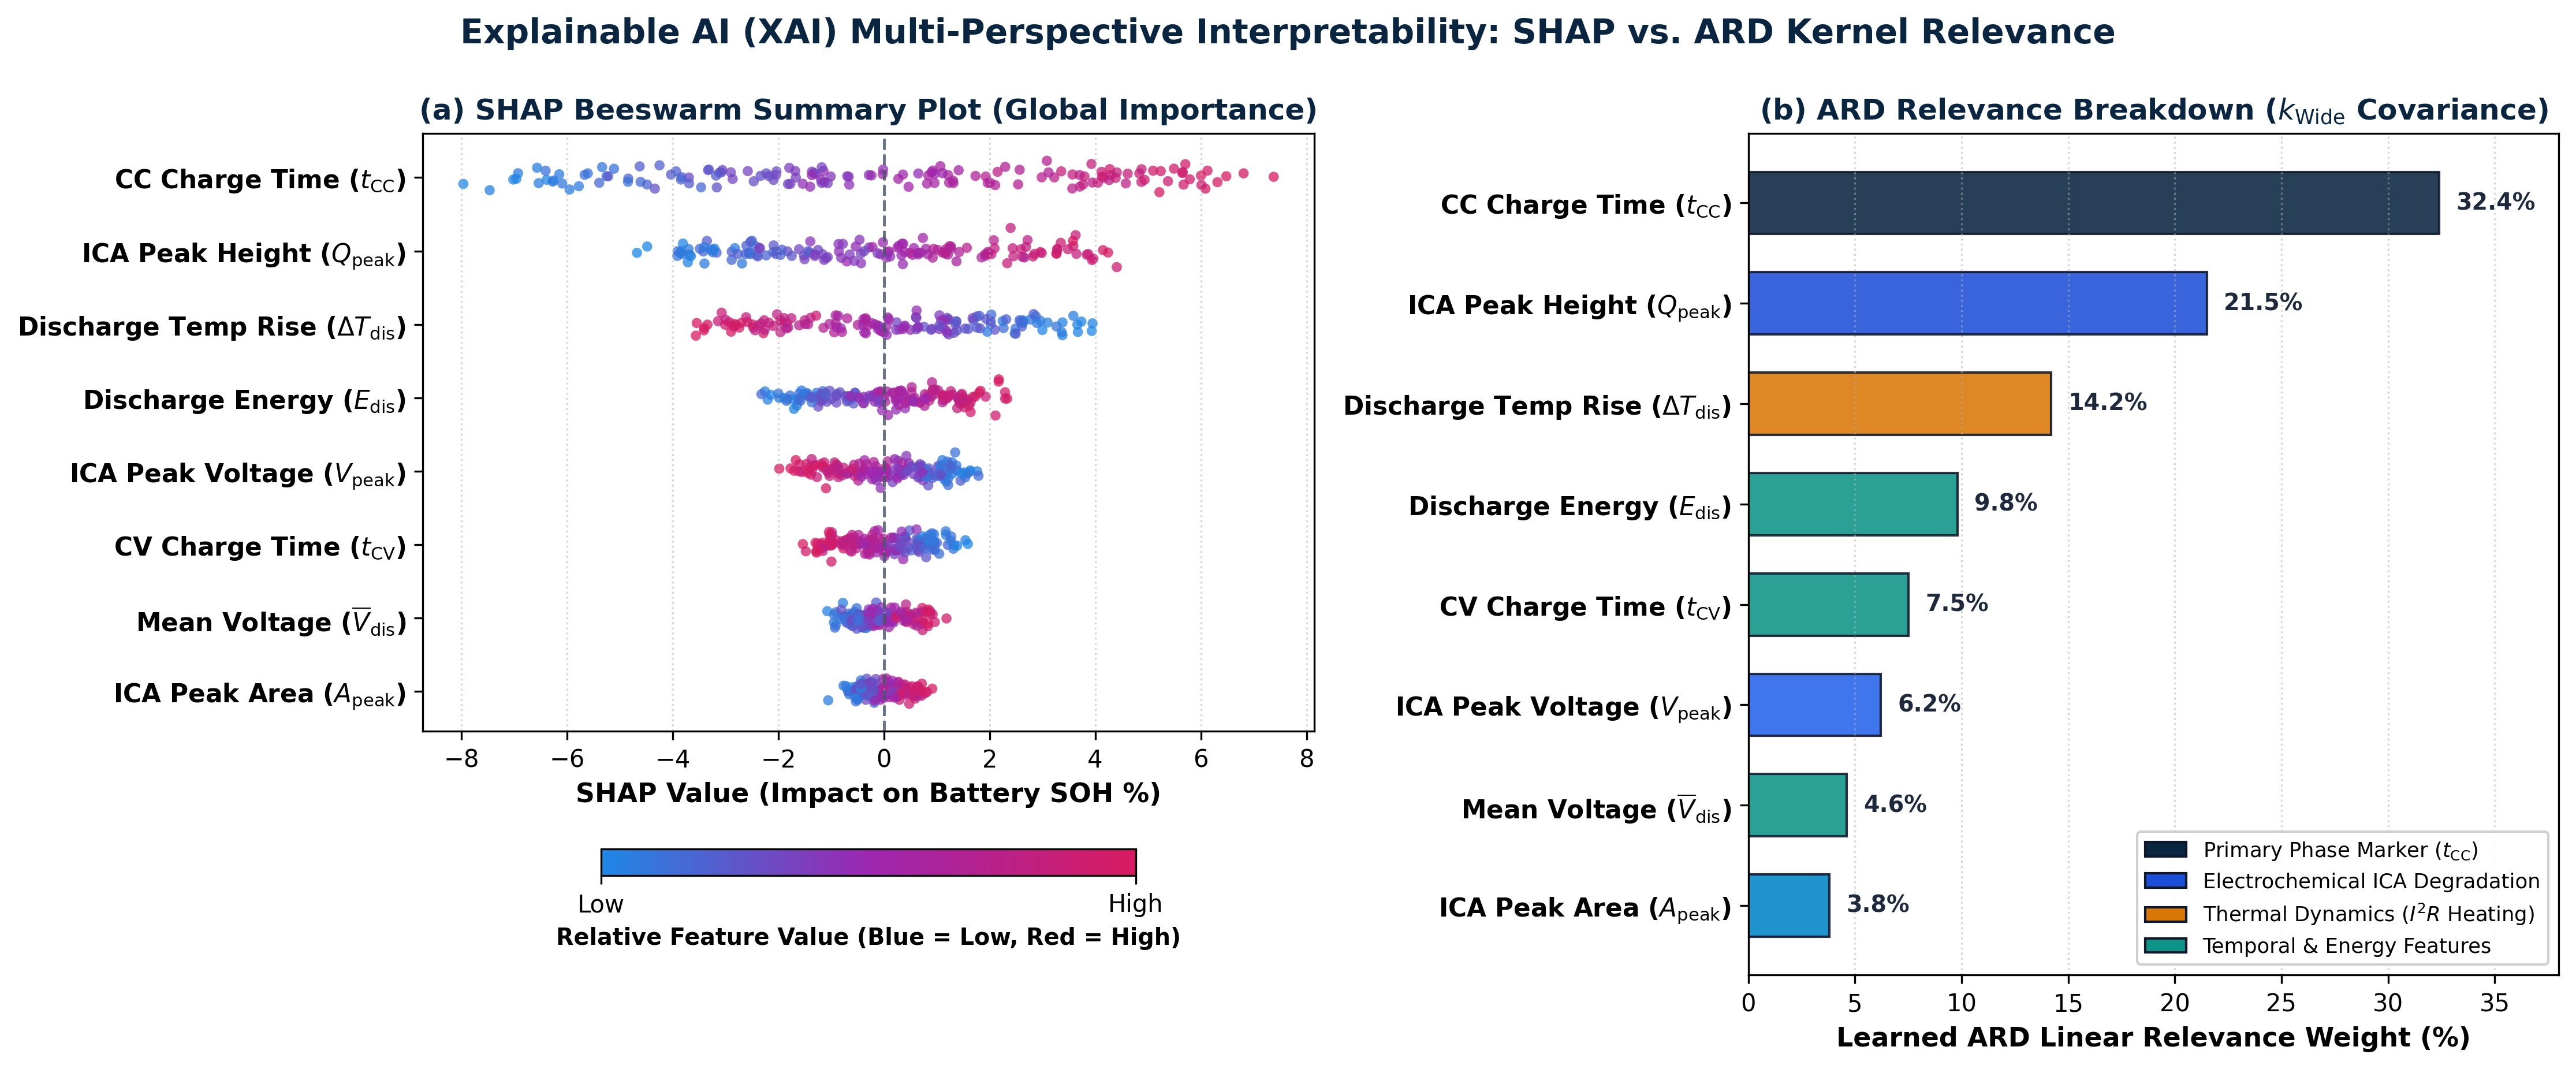
\includegraphics[width=\linewidth]{../../results/poster_assets/xai_insights_grid.png}\\[0.2cm]
    {\footnotesize \textbf{Figure 4:} (a) SHAP beeswarm verifies $t_{\text{CC}}$ and $Q_{\text{peak}}$ as dominant drivers; (b) ARD linear relevance matches electrochemical degradation physics.}
  \end{block}

  \begin{block}{10. Edge AI Benchmarking on NVIDIA Jetson Orin Nano}
    \centering
    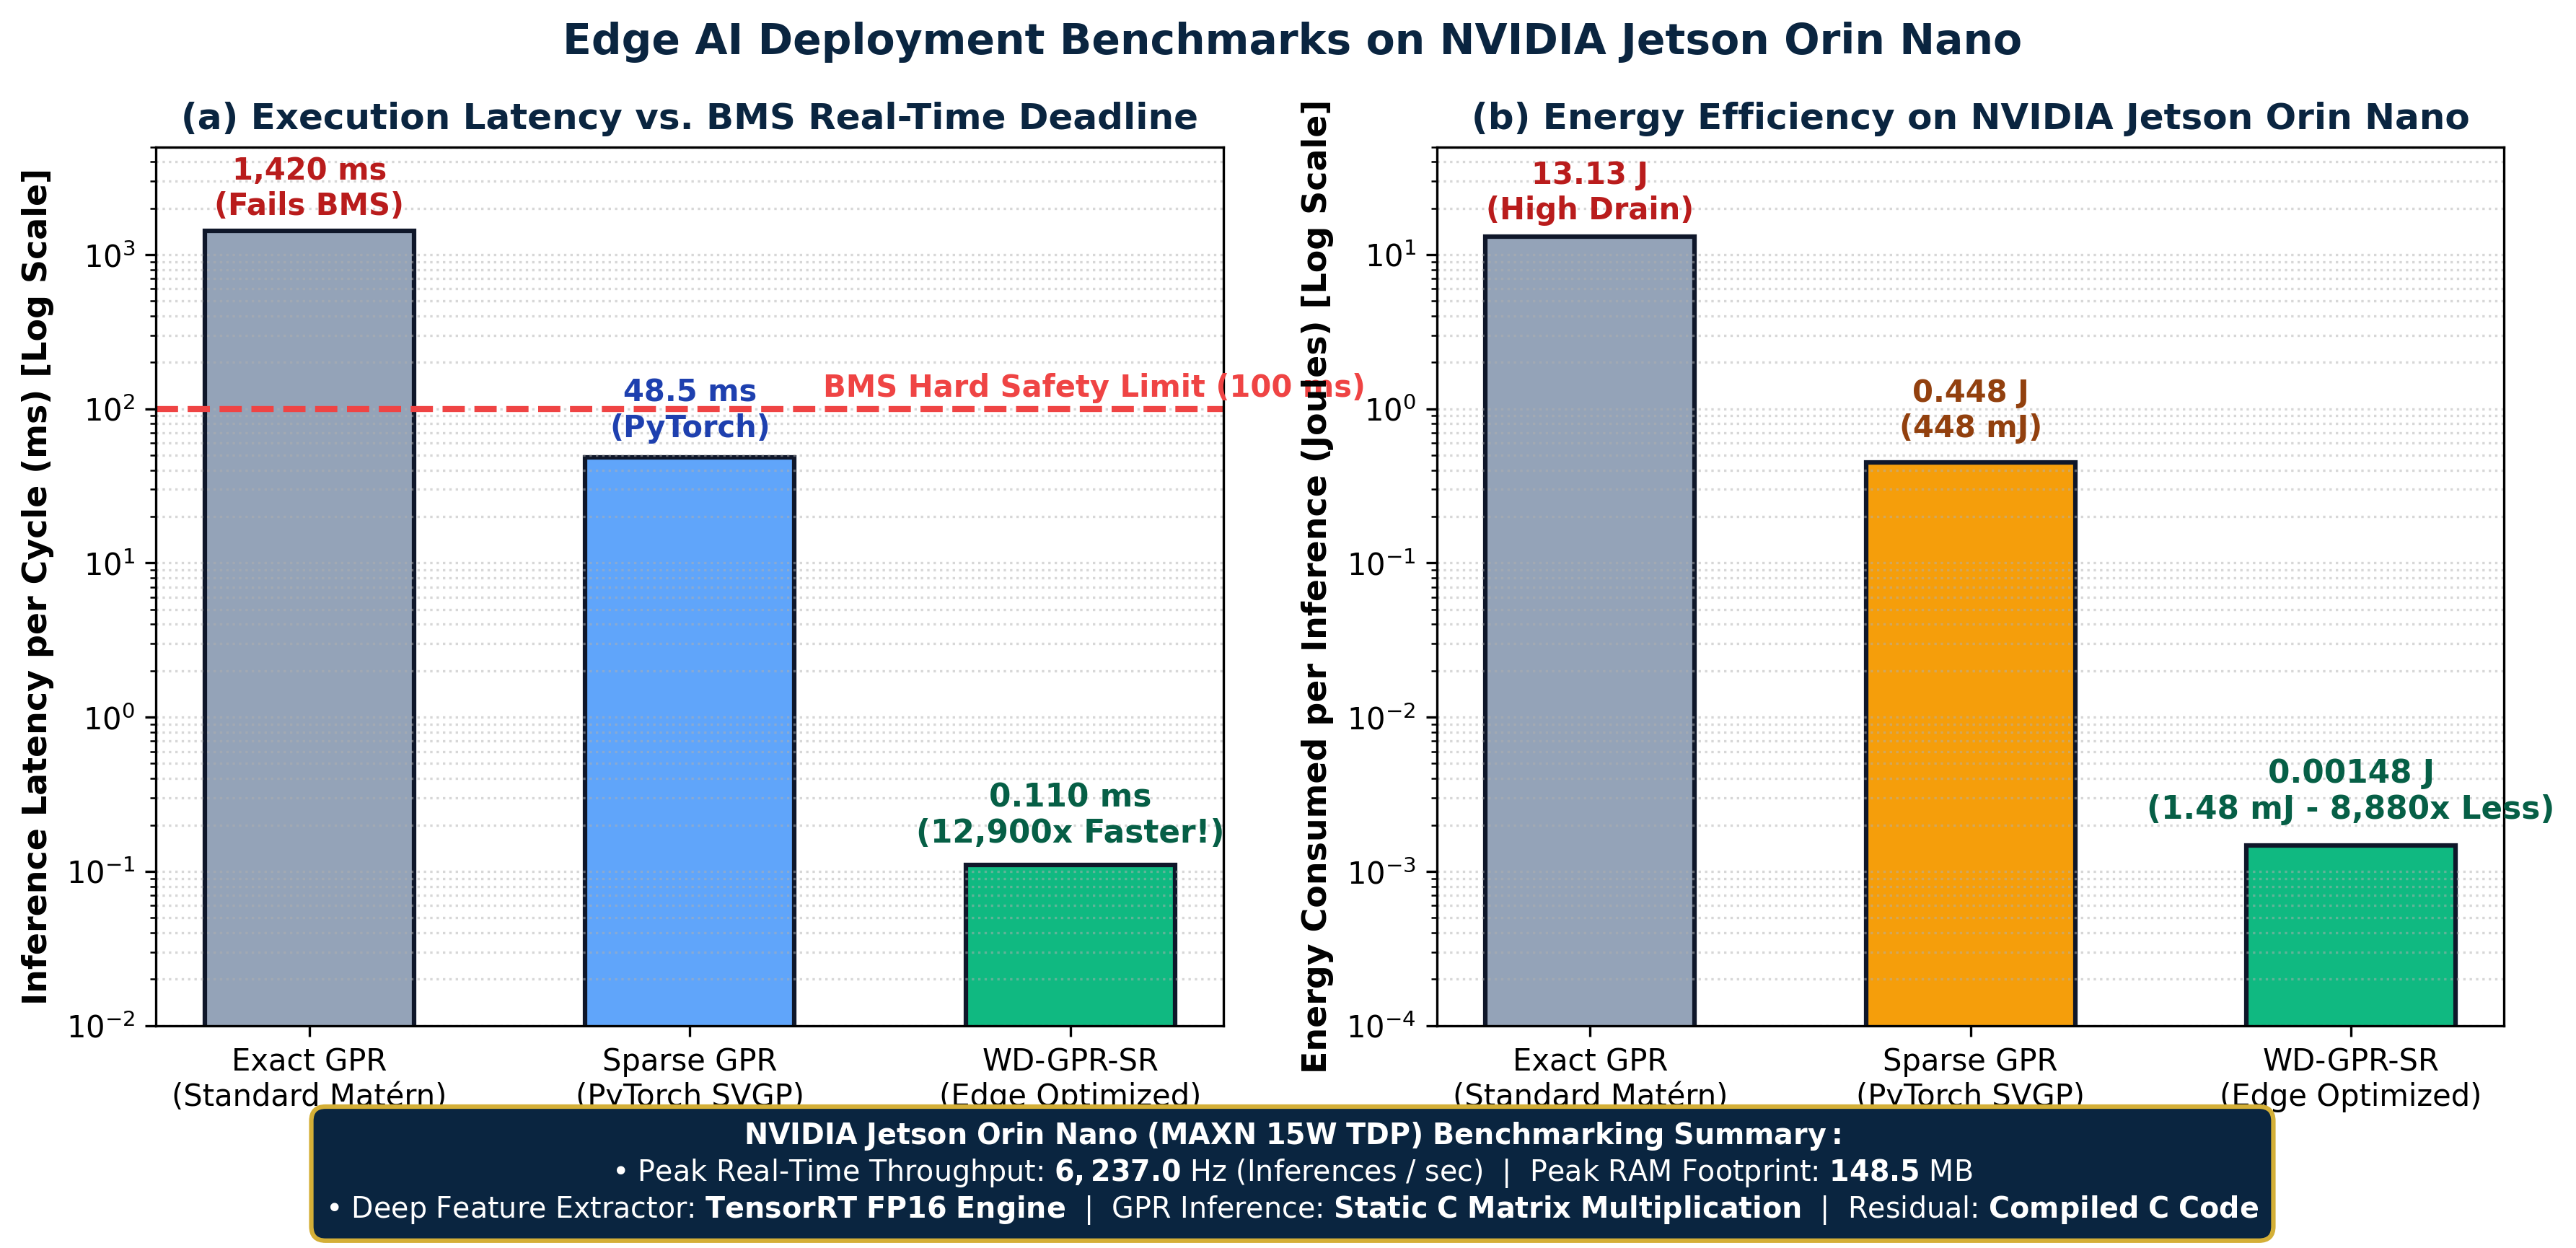
\includegraphics[width=\linewidth]{../../results/poster_assets/edge_deployment_metrics.png}\\[0.2cm]
    \begin{tcolorbox}[colback=green!10,colframe=green!50!black,arc=2mm,boxrule=1pt]
      {\footnotesize \textbf{Hardware Certification:} \textbf{0.110 ms} median latency (6,237 FPS) and \textbf{1.48 mJ} per inference, providing a \textbf{12,900$\times$ speedup} and \textbf{8,880$\times$ energy reduction} over standard GPR, well within the 100 ms BMS limit with 148.5 MB RAM footprint.}
    \end{tcolorbox}
  \end{block}

\end{column}

\end{columns}

\end{frame}
\end{document}

